\documentclass[a4paper,serif]{rpg-module}
\usepackage[utf8]{inputenc}
\usepackage{microtype}
\usepackage{graphicx}
\usepackage{wrapfig}
\usepackage{units}
\usepackage{booktabs}
\usepackage[labelfont=bf]{caption}
% allow non-hyphenating dashes like in AC~\=/1 (AC -1)
\usepackage[shortcuts]{extdash}

% list only sections for the table of contents
% \setcounter{tocdepth}{1}

% Clickable hyperlinks
\usepackage{hyperref}
\hypersetup{colorlinks, linkcolor=blue}

% use dash for items
\renewcommand{\labelitemi}{$-$}

\title{\textbf{Raising a God}}
\author{Alex Schröder}

\begin{document}

\title{Raising a God}
\author{Alex Schroeder}
\titlerunning{Raising a God}
\subtitle{A campaign setting for character levels 5--10}
\coverimage{Floating-Island.jpg}

\abstract{This is a mini-campaign for players in their mid levels,
  levels five to ten. Player characters start looking for a place to
  build their castles and tower, thieves look to expand their network
  of spies and thieves, clerics start meddling in the affairs of the
  gods. Some of long term goals players might have: end the slave
  trade on Hinia Oot; raise the dead god of light, Arden; topple the
  reign of the grey elf witch Susrael; prevent the rise of the demon
  lord Tsathoggua.}

\copyrightblock{This module is
  \href{https://creativecommons.org/publicdomain/zero/1.0/deed}{dedicated
    to the public domain}.}

\contactblock{% column 1: logo
  \begin{center}
    \includegraphics[width=2cm]{OSR.png}
  \end{center}
}{
  \vspace{0.5cm}
  This module provides stats compatible with any classic role-playing
  game by the \emph{Old School Renaissance} (OSR).
}{
  \vspace{0.4cm}
  \begin{flushright}
    Alex Schroeder can be reached by email:
    \href{mailto:kensanata@gmail.com}{kensanata@gmail.com}
  \end{flushright}
}

\maketitle

% (query-replace-regexp "\\b\\([A-Z][A-Z]\\) \\b" "\\1~")
% AC 5
% (query-replace-regexp "\\([0-9,]+\\) ?\\(h\\|min\\|s\\|ft\\|gold\\)\\b" "\\\\unit[\\1]{\\2}")
% 1h 30ft 10 gold
% (query-replace-regexp "\\([0-9]\\{1,3\\}\\)\\([0-9]\\{3\\}\\)\\b" "\\1,\\2")
% 100 1000 10000 100000 but these require multiple calls: 1000000 10000000 
% (while (re-search-forward ".\\{71\\}" nil t) (fill-paragraph))

\part{Gods \& Demons}

The gods and demons are important because characters will able to
visit their \emph{halls}. These can be reached by secret \emph{gates}
when sailing the \emph{Astral Sea} when climbing the branches of the
\emph{World Tree} connecting all the planes of existence.

There is a chance that the gods will send one of their agents to help
if their name is called. In order to succeed, players need to keep
track of \textbf{a score for each god} they care about. As characters
do things to honor or spite the various gods, their score goes up.
This could be about saving or killing their followers, building altars
and temple in their name, defiling their altars or acting on visions
sent by them. This score is the percent chance that the god will act
when their name is called. Whether the agents appearing will in fact
help the characters depends on their past actions. An evil demon lord
like Set might still send a naga to help a paladin of Mitra, hoping to
mess with them.

When paladins and clerics cast \textbf{spells of level four and
  higher}, the spell effect usually involves the appearance of such an
agent, and an opportunity for some discourse.

\section{Freya and Odin}

Freya is the goddess of winter, of spring, of fertility, of grain, of
war, of cats and boars, of magic. She leads the valkyries and collects
half the slain in battle. These dine with her in \emph{Sessrúmnir},
her hall in Asgard.

Odin is the god of wisdom, of magic and poetry, of war, of eagles and
ravens, of runes, of wanderers. He wields a magic spear, he raises the
dead, he rides an eight legged horse called Draupnir. The other half
of the slain in battle dine with him in \emph{Valhalla}, his hall in
Asgard.

In times of need, both of them will send a \textbf{valkyrie} named
\textit{War}, \textit{Mercy} \textit{Spear}, \textit{Cruel} or
\textit{Fight}: HD~6 AC~2 1d8 \textit{sword+3} MV~18 ML~12 XP~820,
flying, only harmed by magic or magic weapons. The swords of valkyries
are bright swords of light. When swinging such a sword, the wielder is
compelled to shout for blood and glory at the top of their voice.
Also, when allies are fighting, the owner of such a sword is compelled
to draw it and join this melee. When resisting such a compel for the
third time, the sword looses its magic. The owner is considered unfit
to wield it.

\section{Loki}

Loki is the god of lies, of deceit, of misdeeds, of excuses and
explanations, of looking the other way, of tricksters, thieves and
shape changers, a friend of giants, the innocently accused, the
misunderstood and the innocent. He can be found brooding in his hall
\emph{Ethrahell} in Utgard.

In times of need, he might send a nameless \textbf{shape changer}: HD
4 AC~5 1d12 MV~9 ML~10 XP~190, \textit{polymorph} at will, immune to
\textit{sleep} and \textit{charms}. Clearly, mostly useful when in
need of deception.

\section{Mitra}

Mitra is the goddess of law, of fire, of bulls, of contracts, of
bonds, the swearing of oaths, of honesty and truth, of loyalty and
sacrifice for the community. Her hall is built atop a lake of fire
deep underground in Muspelheim and called \emph{Eldivatn}.

In times of need, she might send a \textbf{minotaur} named
\textit{Silence}, \textit{Calm}, \textit{Truth Teller} or
\textit{Spirit Guide}: HD~6 AC~6 1d6/1d6 MV~12 ML~12 XP~820,
\textit{mesmerize} any listeners at will (listeners must save vs.
spells or stop hostilities speak nothing but the truth), immune to
\textit{sleep} and \textit{charms}.

\section{Set}

Set is the demon lord of snakes and crocodiles, of assassins, of
revenge, of spies and diplomats, of poison makers, of death traps, of
hypnotists and mind benders. His hall is the subterranean
\emph{Eiterhorg} in Svartalfheim.

In times of need he will send a \textbf{naga} named \textit{Sweet
  Stab}, \textit{Revenge}, \textit{Crocodile Tears} or \textit{Coral
  Death}: HD~9 AC~7 1d8 \textit{poison} MV~6 ML~12 XP~2,400,
\textit{fireball} (7d6) 3/day, \textit{charm person} at will, only
harmed by magic or magic weapons.

\section{Pazuzu}

Pazuzu is the demon lord of pestilence, of miscarriage, of famine and
disease, of crows and vultures, of temptation and betrayal. His tower
\emph{Sandstein} was built in Vanaheim.

In times of need he will send a \textbf{vulture demon} named
\textit{Gangrene}, \textit{Pestilence}, \textit{Corpse Eater} or
\textit{Baby Killer}: HD~8+1 AC~5 1d4/1d4/1d6/1d6/1d8 MV~18 ML~11 XP
2,420, flying, only harmed by magic or magic weapons.

\section{Marduk}

Marduk is the god of war and monster slaying, of armies, of generals,
of brute force. His castle \emph{Unugal} is built in Midgard, the
world of men.

In times of need he will send a \textbf{hunter general} named
\textit{Death}, \textit{Strength}, \textit{Smasher} or \textit{Taker
  of Heads}: HD~6+1 AC~7 1d6 MV~12 ML~12 XP 380, leading a
\emph{hundertschaft}, one hundred \textbf{light infantery}: HD~1 AC~7
1d6 MV~12 ML~10 XP 15. Since there are so many of them, do not forget
to roll a morale check when indicated!

\newpage

\part{Astral Sea}

The Astral Sea is an air filled plane, black and silent. It can be
sailed by flying ships. There are many \textit{gates} in the Astral
Sea, connecting it to many other planes.

%% \begin{figure*}[ht]
%%   \centering
%%   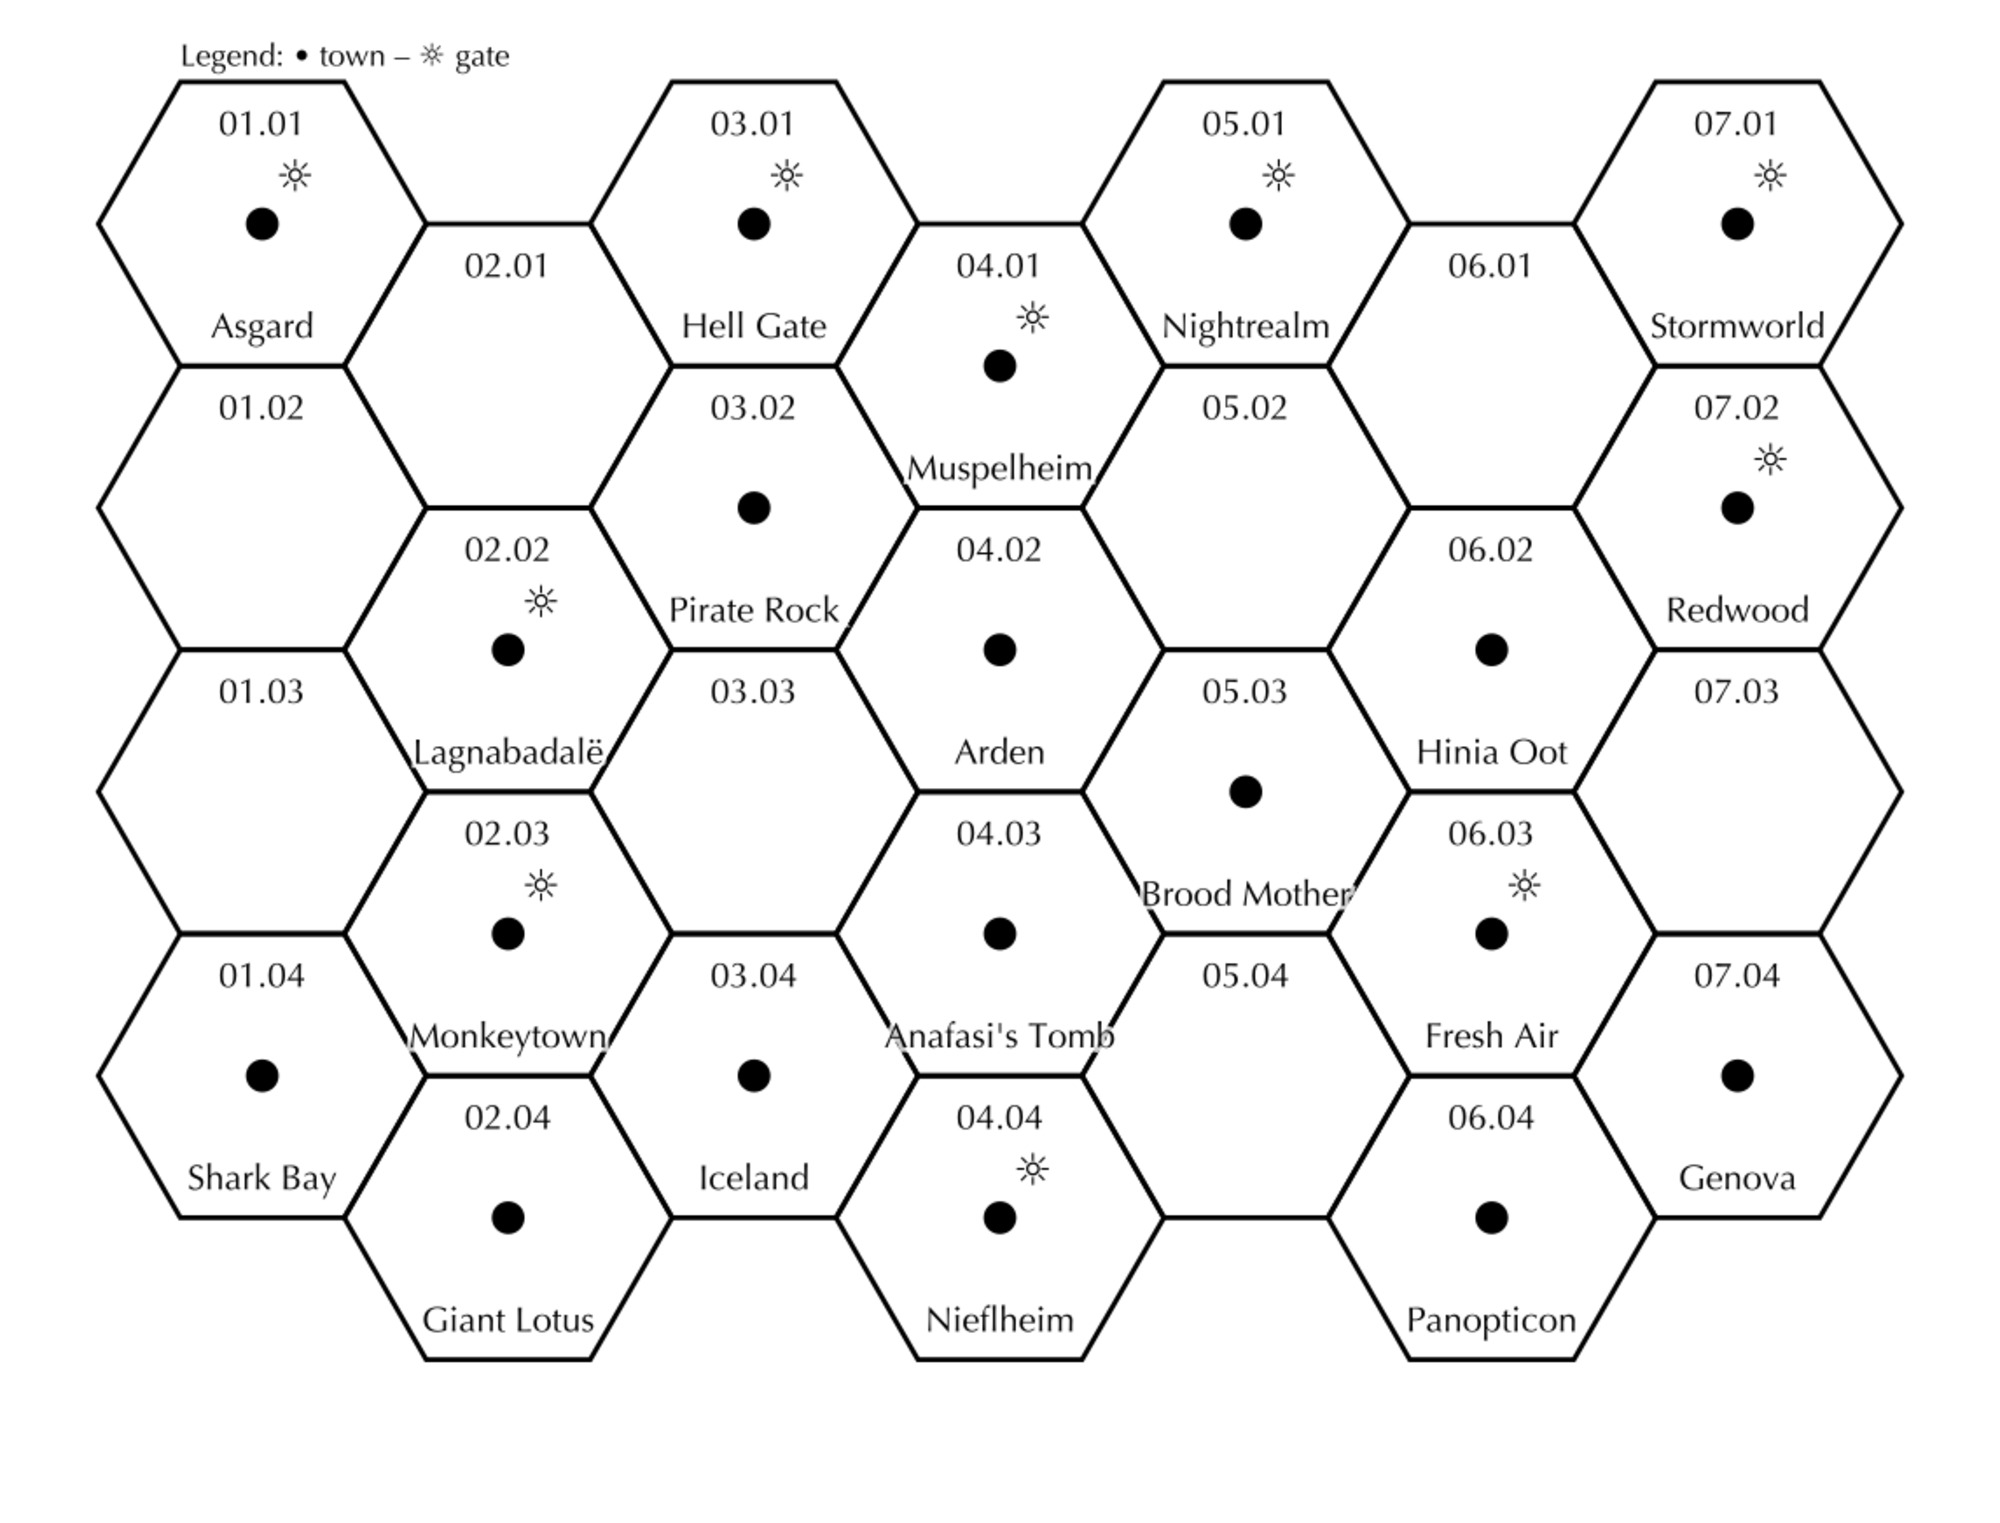
\includegraphics[height=10cm]{Astral-Sea.jpg}
%%   \caption{The Astral Sea can be sailed by flying ships.}
%% \end{figure*}

\section{Rumors}

\begin{itemize}
\item Asteroids fly through the darkness, their caverns and craters
  filled with vampires and ghouls
\item There are islands bearing life floating in the Astral Sea
\item All life clings to \textit{portals} of one sort or another
\item Perhaps light and warmth spills over from a plane of eternal
  fire such as Muspelheim, or from glowing plants or stones
\item There are people who can summon and control \textit{astral
  whales} and \textit{sky squids}
\end{itemize}

\section{Encounters}

With a flying ship, travel from one hex to the next takes about a day.
Roll once per day.

\begin{center}
\begin{tabular}{cl}
\tableheader[b]{1d10 & Ship Encounter}
1 & \hyperref[sec:monkeyman-caravel]{monkeyman caravel}, see p.~\pageref{sec:monkeyman-caravel} \\
2 & \hyperref[sec:squidman-nautilus]{squidman nautilus}, see p.~\pageref{sec:squidman-nautilus} \\
3 & \hyperref[sec:eelman-centipede]{eelman centipede}, see p.~\pageref{sec:eelman-centipede}    \\
4 & \hyperref[sec:void-pirate-pike]{void pirate pike}, see p.~\pageref{sec:void-pirate-pike}    \\
5 & \hyperref[sec:vampire-deathrock]{vampire deathrock}, see p.~\pageref{sec:vampire-deathrock} \\
6 & \hyperref[sec:sharkman-hammer]{sharkman hammer}, see p.~\pageref{sec:sharkman-hammer}       \\
7 & \hyperref[sec:astral-whales]{astral whales}, see p.~\pageref{sec:astral-whales}    \\
8 & \hyperref[sec:sky-squids]{sky squids}, see p.~\pageref{sec:sky-squids}             \\
9 & \hyperref[sec:asteroid-field]{asteroid field}, see p.~\pageref{sec:asteroid-field} \\
10 & \hyperref[sec:rainbow-nebula]{rainbow nebula}, see p.~\pageref{sec:rainbow-nebula} \\
\end{tabular}
\end{center}

\section{Ship Combat}
\label{sec:ship-combat}

The \textit{Labyrinth Lord} rules cover ship combat. The
\textit{Spelljammer} rules have even more ship combat rules. Here's a
simple alternative. Ships have hit points and armor class. When a
\textbf{catapult} is manned by 4 crew, it takes four rounds to reload
(\textit{rate of fire} is 5), it attacks as a fighter level 4 and it
does 3d6 damage. Use one roll to attack the ship and a target person
visible on deck, if any. If the roll hits, apply damage. If there is a
second target person nearby, it is automatically targeted as well.
Ordinary weapons cannot damage a ship.

When a ship is brought to zero hit points and every time it is hit
thereafter it takes critical damage. Roll 1d8:

\begin{enumerate}
\item spectacular explosion, all is gone, everybody takes an extra 5d6
\item slow motion breaking up of the ship, everything is gone but the
  crew is unharmed
\item ship breaks into several pieces, everything is broken but
  lifeboats or the like can be fixed in an hour
\item a disabling hit, immobilizing the ship, all infrastructure
  breaks down, no more catapult use
\item fire breaks out and spreads unless five crew deal with it for
  half an hour
\item a gaping hole in the hull immobilizes the ship and provides a
  extra ingress for boarders
\item a crippling shot immobilizes the ship, taking down mast and
  rigging, destroying oars and the like
\item the hit reduces the ship's speed as a mast, sail or some oars
  are taken out; no fleeing from the scene
\end{enumerate}

\textbf{When a ship tries to run}, roll 2d6, +1 if the fleeing ship is
significantly smaller than the pursuing ship. On a 10+, you get away
because of some lucky shots discouraging your enemies, or because you
dove into an asteroid field, or because you managed to make it into a
nebula. On a 7--9, you get away but the ship takes damage
necessitating a lengthy overhaul in a shipyard. Perhaps you smashed
into some asteroids or you took a few hits from parting shots. On a
6+, you did not make it. Fight to the bitter end or surrender now.

\subsection{Monkeyman Caravel}
\label{sec:monkeyman-caravel}

"Monkeymen" is what other people call humans – humanoids with monkey
heads. A caravel is a small trading ship made of wood with a single
catapult and 10 crew. HP~20 AC~9 3d8.

The prize usually consists of ten tons of pickled lotus flesh, wooden
planks, grains and wine barrels, cactus figs, fungus lanterns, or some
other produce worth 1d4 × \unit[10,000]{gold} and the ship itself is
worth another \unit[10,000]{gold}. Clearly, being a pirate is
lucrative.

\subsection{Squidman Nautilus}
\label{sec:squidman-nautilus}

This is a slaver ship built atop a trained nautilus with two mounted
catapults. The crew consists of squidmen, charmed slaves manning two
catapults and intelligent giant spiders. The shell provides excellent
protection. HP~35 AC~2 3d8/3d8.

The nautilus' ten \textbf{tentacles} are used to pick up victims and
deliver them into the slave hold. Each tentacle acts as a separate
creature. HD~1 AC~2 1d4 MV~3 ML~10 XP~13; when hit, save vs. poison or
be \textit{paralyzed} for \unit[10]{min}.

The five \textbf{squidmen} have terrible psi powers but they are
cowards. HD~7+1 AC~8 1d6 F7 MV~12 ML~6 XP~1,300; \textit{mind blast}
at will stuns anybody they can see within \unit[60]{ft} unless they
save vs. paralysis; \textit{charm person} at will to make slaves
docile unless they save vs. spells; \textit{read thoughts} lets them
read any thoughts within \unit[60]{ft}. If they sing their song of
summoning into the void for \unit[10]{min}, they will call forth a
\hyperref[sec:sky-squids]{sky squid}, see p.~\pageref{sec:sky-squids}.

The fifteen \textbf{slaves} are humans manning the catapults and
repairing damage. HD~1 AC~9 1d6 F1 MV~12 ML~6 XP~10.

The ten \textbf{giant spiders} trained to paralyze victims and drag
them back to their masters. HD~4+1 AC~5 1d8 F2 MV~12 ML~8 XP~215; when
bitten, save vs. paralysis or drop into a death-like trance for
\unit[6]{h}; they can jump for \unit[20]{ft} and get +1 to hit when
they do. They speak of hunting and feeding.

There is a 1 in 6 chance that this slaver ship is actually on the way
back to Hinia Oot and its hold is filled with fifty \textbf{slaves}.
As these would be sold for \unit[25,000]{gold}, freeing them would be
worth as many XP. The ship itself is worth \unit[35,000]{gold}.

\subsection{Eelman Centipede}
\label{sec:eelman-centipede}

This is also a slaver ship built into what looks like a gargantuan
centipede. The crew consists of eelmen manning three catapults or
riding their giant dream beetles. The centipede's exoskeleton provides
good protection. HP~50 AC~3 3d8/3d8/3d8.

The twenty \textbf{eelmen} are a bit like plum colored, eight legged
morays with two skinny arms and a huge teeth filled mouth, armed with
a spear and long daggers: HD~4 AC~7 1d6 F4 MV~9 ML~10 XP~135.

The eel men are cowards and fear combat, but they have each tamed ten
\textbf{giant dream beetles} with iridescent cobalt blue wings: HD~4
AC~3 2d6 F2 MV~6 ML~9 XP~135. Whenever the beetles move, their wings
\textit{bedazzle} anybody who sees them: save vs. paralysis or spend
your next round standing and drooling. The eel men have a
\textit{poison stinger} they'll use on bedazzled foes: it causes
paralysis for \unit[1]{h}, no save. Closing your eyes avoids
bedazzlement gives -4 to hit.

There are special polarized goggles made by sharkmen that prevent
bedazzlement without giving you penalties, but they keep this secret
to themselves. It's why the sharkmen are never attacked by eelmen,
though.

There is a 1 in 6 chance that this slaver ship is actually on the way
to Hinia Oot and its hold is filled with fifty \textbf{slaves}. As
these would be sold for \unit[25,000]{gold}, freeing them would be
worth as many XP. The ship itself is worth \unit[50,000]{gold}.

\subsection{Void Pirate Pike}
\label{sec:void-pirate-pike}

A ship shaped like a fish with an open deck, no catapults and twenty
elven pirates. The deck is protected by a row of mounted shields.
HP~20 AC~8.

The greedy pirate \textbf{gray elves} are eager to surprise you with
their spells: hp~1d6 AC~5 1d6 E1 MV~12 ML~8 XP~6; \emph{magic missile}
1/day. Their \textbf{invisible captain}: hp~3d6 AC~5 1d6 E3 MV~12 ML~8
XP~65; \emph{magic missile}, \emph{detect magic}, \emph{invisible}.

They're not interested slaves, they just care for the loot. Their
ruler is trying to find allies against Susrael. The ship is worth
\unit[20,000]{gold}.

\subsection{Deathrock with Vampires}
\label{sec:vampire-deathrock}

Deathrocks are hurtling through the Astral Sea at slow speeds. They
are densely packed with ghouls, waiting for it to make contact with
the living. A deathrock is easy to avoid if you're on a ship and using
a spy glass. By the time the unaided eye sees the packed ghouls eager
to launch themselves from the rock with their catapults, it is already
too late.

A typical deathrock has about 500 \textbf{ghouls}. HD~2 AC~6
1d4/1d4/1d4 F2 ML~9 MV~9 XP~47; when they hit, save vs.~paralysis
unless you're an elf or be paralyed for \unit[1]{h}; the slain will
rise as ghouls.

The ghouls are ruled by a dozen \textbf{vampires}. HD~9 AC~2 1d10
MV~18 ML~11 XP~7,300; immune to immune to \textit{sleep},
\textit{hold}, \textit{charms} and normal weapons; their hit drains
\emph{two} levels; shape change into a large bat at will; charming
gaze at will; the slain will rise as vampire slaves. When reduced to
zero hit points, they'll turn gaseous and retreat to the central crypt
within the deathrock.

The vampires each wear a crown set with gems and necklaces and
bracelets to match, each set being worth \unit[10,000]{gold}. The
central crypt can only be reached by tiny bats flying through small
tunnels. The coffins stand at the bottom of a cathedral pit
\unit[100]{ft} deep filled with poisonous gas. The vampires, being
already dead, are unaffected.

\subsection{Sharkman Hammer}
\label{sec:sharkman-hammer}

A white ship shaped like a giant shark, no catapults and 
greedy pirate \textbf{gray elves} eager to surprise you with their
spells: hp~1d6 AC~5 1d6 E1 MV~12 ML~8 XP~6; \emph{magic missile}
1/day. Their \textbf{invisible captain}: hp~3d6 AC~5 1d6 E3 MV~12 ML~8
XP~65; \emph{magic missile}, \emph{detect magic}, \emph{invisible}.

They usually kill the crew or let them run. They're not really
involved in the slave trade. They're interested in bringing powerful
characters to their ruler who'll try to set them up against Susrael.

The gray elves are out for loot. The ship is worth
\unit[20,000]{gold}.

\subsection{Astral Whales}
\label{sec:astral-whales}

Astral whales are dream singers the size of cities. Their thoughts
overwhelm all others. Their bodies are like cliffs a thousand feet
high. To hunt them is to use harpoons forged in hell according to
plans devised by titans of war. When you're too close, it's like a
religious experience. If you need to expand the campaign in an
unexpected direction, roll 1d6 and be prepared to spend some time
developing the idea for next session:

\begin{enumerate}
\item your ship is swallowed by the whale; there is a \textbf{city
  full of snail people} bathed in mauve light in here but their queen
  \textit{Patient Seer of the Seven Directions} is weak and a
  triumvirate of martial snail men is trying to change the course of
  the whale's dive in order to swallow and assimilate a large city
  like Genova; these three powerful snails are called \textit{Acid of
    Perfection}, \textit{Eternal Radula of the Mind} and \textit{To
    Crawl Is To Fly}

\item as you gape in wonder, the eddies of the whale dream take hold
  of your ship and pull you over \textbf{to the other side}, a
  parallel \textit{Purple Sea}, much like a \textit{Shadow Land}, but
  colorful, of lonely pink skies and atomic tangerine desert worlds,
  where sorcerer kings have drained all life and nothing but their
  dreams remain, and if you want you can find them still, their
  pyramids and mummies, their desiccated servants and buried boats,
  and if you bring them peace their dreams will end and the Purple Sea
  will fade, the whale will die and you might return to where you came
  from

\item a trail of colors erupt behind the whale, miles and miles of
  chartreuse, of mandarine, of isabelline, of turquoise, of carmine,
  an \textbf{explosion of colors}, of plants gushing forth, a strip of
  land being drawn here from the whale's dream, the \textit{Bridge of
    Dreams} and giving birth to the \textit{Bean People}, green
  humanoids that grow out of your ship's wooden planks over the coming
  hours, \textit{charming} you and all the crew unless they save vs.
  spells, spreading from your ship to others, a tireless appearance of
  messengers of peace and understanding for the next two months with
  names like \textit{Harmless}, \textit{Peace}, \textit{Happiness} or
  \textit{Soft Words}, friendly and caring, no matter how often you
  kill them

\item a \textbf{titan of war} about \unit[200]{ft} high is using his
  \textit{sun lance} to kill the whale as you watch; the pain and fear
  of the dying whale transport you into the titan's nightmare of fire
  where rivers of lava rain down from above and glowing ghost giants
  with spears a mile long destroy cities and their dread gaze
  vaporizes all life—and you know that one of them is the titan of war
  you just saw and if only you could speak to it, to the war titan
  \textit{Rain of Fire}, this madness could end; the alternative is to
  die with the whale, unable to leave his dream maelstrom

\item this whale has been used by a \textbf{lich lord} for a ritual of
  divine transcendence; the entire back of the whale is a gaping
  wound, a flesh pit \unit[500]{ft} wide, trailing black fumes boiling
  up from burning cauldrons of whale fat extracted from the living
  flesh by brass pipes and rusty iron needles, wraith fragments of
  whale soul screaming in madness and pain, going after any living
  being, begging for help, demanding help, spreading madness; and what
  god is being cursed by \textit{Father Bone Forest}? who is being
  consumed and killed by this dread ritual?

\item waves of intense hate and love and fear and joy wash over you
  and suddenly you \textit{understand} and you \textit{know}, for this
  whale is a \textbf{god} and you have been chosen, all of you, this
  ship of yours, you are the chosen ones, the \textit{whale people},
  followers of \textit{Deep Thought}, no save; if you decide to
  abandon your new faith, you'll be a heretic and you know it; and the
  people need you—the whale will use you to transform society and
  right all the wrongs, create a brotherhood of sophonts, a society of
  friends; boons granted include an \textit{aura of peace}, a strong
  \textit{empathy} for all living things and \textit{words of wisdom}
  to calm all angry spirits
\end{enumerate}

\subsection{Sky Squids}
\label{sec:sky-squids}

The \textbf{squidmen} know the songs to summon and anger these
god-like creatures that live between the stars. HD~20 AC~7 8×3d6 4d8
F20 MV~15 ML~10 XP~3,250. When angered, they will happily smash a ship
and proceed to eat the survivors. When found on their own, these sky
squids will only attack if your ship looks like a giant fish.

To learn this song, you must befriend a squidman. To sing the song,
you need to wear a \textit{crown of thought} or you need to have
terrible psi powers.

\subsection{Asteroid Field}
\label{sec:asteroid-field}

Asteroid fields are perfect hideouts for \textbf{pirates}. When flying
into an asteroid field, one flies very slowly or risks loosing a ship.
Giving chase is a dangerous proposition.

\begin{enumerate}
\item The one fleeing starts by announcing a number of risky maneuvers
  they're willing to make.
\item The one pursuing either breaks off the chase or matches the
  number.
\item When matching the number, both parties roll 1d6 of ship damage
  for every risky maneuver they agreed to make. See
  \hyperref[sec:ship-combat]{ship combat} for the table of critical
  damage at zero hit points.
\item The one fleeing either slows down and allows ship
  combat to resume or returns to step \#1.
\end{enumerate}
 
A typical \textbf{pirate stone fortress} has two catapults and two
large longships which are used to raid other settlements. HP~100 AC~2
3d8/3d8 for the fortress and HP~20 AC~8 for the longships.

There will be around 200 \textbf{pirates} in the fortress itself. HD~1
AC~7 1d6 MV~12 ML~6 XP~10.

There are ten \textbf{officers} in plate armor to run the operation.
They will captain ships and lead raids or run the fortress. HD~5 AC~2
1d6 MV~6 XP~200.

A typical longship is worth 20,000~gold, a fortress with a fortified
harbor is worth 100,000~gold (but harder to sell than a ship).

\subsection{Rainbow Nebula}
\label{sec:rainbow-nebula}

Occasionally, there will be 

\newpage

\section{Lagnabadalë}

\begin{figure*}[t]
  \centering
  \includegraphics[draft,width=16cm,height=8cm]{Lagnabadale.png}
\end{figure*}

This is the home of the sea elves ruled by Lady Gerdana. These days a
\textbf{hell barge} is blockading the elven harbor, however. The elves
have fled inland and are hiding in the hills, their fleet destroyed
and their city burned. Defeating the demon will allow the elves to
reconquer their island.

The island itself consists of three major areas: the middle lands with
beautiful beaches and huge boulders. In the north, there is a small
naiad lake surrounded by huge boulders and in the south, where a big
pile of these boulders runs into the sea, a gap between two of them
holds a permanent portal two a primary world. On the other side, a
small settlement of elves lives along a rocky ocean coast. The elves
on both sides of the portal are ruled by Lady Gerdana
and keep the existence of the portal secret from their enemies.

The elves have been thoroughly beaten by the demon and its horde and
the only ones left behind are the ones that didn't make it to the
gate.

\begin{table*}[b]
  \small
  \centering
  \begin{tabular}{cl}
    1d8 & Random Encounters (1/6 per day, 1/6 per night) \\
    \cmidrule(lr){1-1}\cmidrule(lr){2-2}
    1 & 2d4 slow moving, dead baboons, creeping through burnt out villages HD 2 AC 8 1d8 F2 MV 6 ML 6 XP 29 \\
    2 & 1d10 baboons hungry for meat and enjoying the destruction HD 2 AC 6 1d4 F2 ML 8 MV 12 XP 20 \\
    3 & 1d6 giant bats spying for their demonic overlord HD 2 AC 6 1d4 F1 ML 8 MV 18 XP 20 \\
    4 & 1d4 cursed boars, sniffing out survivors, trailing black smoke HD 3 AC 7 1d8 F2 ML 9 MV 15 XP 50 \\
    5 & 2d6 giant boars, covered in festering wounds, hungry for blood HD 5 AC 6 1d12 F5 ML 9 MV 15 XP 200 \\
    6 & 1d4 demonic boars with a charming voice 3×/day and 1d12 slaves HD 9 AC 3 2d6 F9 ML 10 MV 18 XP 3800 \\
    7 & 2d12 elves with no more spells left, trying to reach the portal HD 1+1 AC 5 1d8 E1 ML 8 MV 12 XP 15 \\
    8 & 2d12-1 elves on a rescue mission (\emph{sleep}) for their friend HD 1+1 AC 5 1d8 E1 ML 8 MV 12 XP 15 \\
  \end{tabular}
  \caption{Roaming bands of demonic agents searching for stragglers.
    Demonic boars are only damaged by magic or silver weapons. They
    like to send their slaves ahead. The giant bats will call
    Cheirofrastus when one of their own gets killed. If they spot the
    party, they'll go and attract baboons or cursed boars.}
\end{table*}

\textbf{Cheirofrastus} the boar-headed demon rules this place,
shrouded in permanent \emph{darkness} that only he can see through
(attack at -4), appearing wherever he wills at a moment's notice,
causing a dreadful \emph{fear} wherever he goes (save vs. spells to
resist), can only be hurt by magic weapons +1 and spells, being able
to cloud reality in an \emph{illusion} at will (save vs. spells to
disbelieve if and only if touching it), to \emph{read thoughts} and
speak in \emph{tongues}, able to change into a giant flying black
boar-headed snake dripping caustic green vapors when angered (AC~\=/1,
tail slap 2d8, bite 4d8, suffer 1d8 damage by the gas when inside the
darkness surrounding the demon).

The main agents of the demon's appetite for destruction are hundreds
of demonic animal agents roaming the island.

The ruins of the elven settlement house eight \textbf{wights}.

The foul forest has been taken over by a gang of \textbf{werewolves}.

\subsection{The Book of the Sea}
\label{sec:book-of-the-sea}

Lady Geradana has ruled the coastal elves of Lagnabadalë for over 250
years. This is her spell book. These are very traditional spells.

\begin{table*}[!ht]
  \small
  \centering
  \begin{tabular}{cll}
    Circle & Spell Name & Traditional Name \\
    \cmidrule(lr){1-1}\cmidrule(lr){2-2}\cmidrule(lr){3-3}
    1 & Secrets of the Elven Voice & \emph{charm person} \\
    1 & Rune Magic of Our Elders & \emph{read magic} \\
    1 & Drowzy Lull of Waves & \emph{sleep} \\
    2 & Searching My Feelings & \emph{ESP} \\
    2 & Eternal Starlight & \emph{continual light} \\
    2 & The Language of Fish & \emph{speak with animals} \\
    3 & Lightning Storm & \emph{lightning bolt} \\
    3 & Secrets of Whales & \emph{water breathing} \\
    3 & Eye of the Storm & \emph{protection from normal missiles} \\
    4 & Shape Changing & \emph{polymorph}\\
    4 & Banes and Boons & \emph{remove curse} \\
    4 & Flash Flood & new spell \\
    5 & Supremacy of the Will & \emph{telekinesis} \\
    5 & Summon Living Storm & \emph{conjure elemental} \\
  \end{tabular}
\end{table*}

When \emph{water breathing}, you can speak the language of whales.

As is typical for elves, her favorite shape to \emph{polymorph} into
is a blue dragon. At level 9, its stats are AC~0 1d6+1/1d6+1/3d10
MV~24; at level 10 its stats are AC~\=/1 1d8/1d8/4d8 MV~24.

A \emph{flash flood} will create a sudden flood from a body of water
within \unit[30]{ft}. Anybody caught by it must save vs.~death or be
swept away. If wearing metal armor, save vs.~death again or drown
within a minute or two.
  
When \emph{conjuring an elemental}, she prefers to summon an air
elemental called \emph{Flying Debris}, HD~16 AC~-2 3d8 F16 MV~36; plus
1d8 vs.~flying creatures; requires a save vs.~death to approach;
immune to non-magical weapons; will attack summoner and remain on this
plane if the conjurer's concentration fails.

\newpage

\tableofcontents

\end{document}

% Local Variables:
%   eval: (flyspell-mode 1)
%   ispell-local-dictionary: "american"
% End:
